% General beamer options %
%%%%%%%%%%%%%%%%%%%%%%%%%%

%\documentclass[handout]{beamer} % activar esta para imprimir handouts, desactivar la de abajo, y desactivar shownotes (sin overlays)

\documentclass[]{beamer} % para presentaciones

% Class options include: notes, notesonly, handout, trans,
%                        hidesubsections, shadesubsections,
%                        inrow, blue, red, grey, brown

%\usepackage{pgfpages} %This is needed for notes presentation con dual monitor
%\setbeameroption{show notes on second screen=left} % para presentaciones con dual monitor

%\setbeameroption{show notes}  % muestra notas de presentacion intercaladas a las slides
%\setbeameroption{show only notes} % crea documento solo con notas
\setbeamerfont{note page}{size=\tiny} % achica tamaño letra notas (default: small)

% Theme for beamer presentation.
\usepackage{beamerthemesplit}

	% para cambiar el color del theme
	\definecolor{mycolor}{RGB}{203,129,0} % para definir color personalizado, luego reemplazar abajo (ej bg=mycolor)
	\setbeamercolor*{palette primary}{use=structure,fg=white,bg=mycolor}


% Other themes include: beamerthemebars, beamerthemelined,
%                       beamerthemetree, beamerthemetreebars


\setbeamercovered{transparent} % esto hace que las transiciones entre items sean transparentes

%\setbeamertemplate{footline}[frame number] % for inserting page numbers, but in this theme eliminates the whole footer (!)

% This is a macro for inserting page numbers without eliminating the footer

\newcommand*\oldmacro{}%
\let\oldmacro\insertshorttitle%
\renewcommand*\insertshorttitle{%
  \oldmacro\hfill%
  \insertframenumber\,/\,\inserttotalframenumber}
\usepackage{graphicx}

% Other latex useful options
%---------------------------

\usepackage{mathtools}   % loads »amsmath« , for equations
\usepackage{textgreek} % para poder escribir caracteres griegos en el texto sin pasar a mathmode
\usepackage[utf8]{inputenc}  % permite escribir acentos directamente. PERO: asegurarse que en caso de colaboración el colaborador tenga opción utf8 predeterminada en su editor de LATEX ... si no, no funciona
\usepackage{booktabs,dcolumn}% tablas
\usepackage{outlines} % permite mayor flexibilidad en algunas listas
\usepackage{listings} % como verbatim pero permite quebrar líneas (lo que no hace verbatim)
\lstset{
   breaklines=true
    , basicstyle=\ttfamily}  % opción de lo anterior
\usepackage{courier} % para que listings salga en courier, como default verbatim

\usepackage{setspace}
\renewcommand{\baselinestretch}{1}

% Define information for the title page %
%%%%%%%%%%%%%%%%%%%%%%%%%%%%%%%%%%%%%%%%%

\title[Multinivel - ISUC 2018] % this is the reduced title for the foots
{\textsc{\large{1.Introducción}}}

\subtitle{Modelos Multinivel}

\author[Juan Carlos Castillo - jc-castillo.com] % this is the reduced author for the foot
{{Juan Carlos Castillo}}

\institute{Instituto de Sociología \\
Facultad de Ciencias Sociales - Pontificia Universidad Católica de Chile }

\date {\begin{tiny}
14 Marzo 2018 % {\today} %, for today date
\end{tiny}}

             % Enter the date or \today between curly braces


% BEGIN PRESENTATION %
%%%%%%%%%%%%%%%%%%%%%%

\begin{document}

% Creates title page of slide show using above information

\begin{frame}[plain,label=firstframe] % plain is for removing the bars from the top & the bottom in this title slide
  \titlepage
\end{frame}
\note[itemize]{
\item X
}

%\section[Outline]{}  % removed because I did not wanted it to be in the sections menu at the top

% Creates table of contents slide incorporating all \section and \subsection commands

%\begin{frame}
%	\frametitle{Contents}
%  \tableofcontents
%\end{frame}

	\begin{frame}%[allowframebreaks]{Outline}
		\frametitle{Preguntas}
		\begin{itemize}%[<+->] % este signo al lado del itemize es para las transiciones entre items
			\item ¿Qué es un problema de investigación multinivel?
			\item ¿Cuál es la relación entre problemas multinivel y sociología?
			\item ¿Cómo modelar un problema de investigación multinivel?
		\end{itemize}
	\end{frame}

\begin{frame}%[allowframebreaks]%[fragile]{Outline}
	\frametitle{Presentación y programa}

\end{frame}

\begin{frame}%[allowframebreaks]{Outline}
	\frametitle{Contenidos}
	\begin{minipage}{\textwidth} % con esta instruccion para ajustar espacio entre líneas
		\tableofcontents %  [currentsection,currentsubsection]
	\end{minipage}
\end{frame}

\section{Marco general}

\begin{frame}%[allowframebreaks]{Outline}
	\frametitle{Contenidos}
	\begin{minipage}{\textwidth} % con esta instruccion para ajustar espacio entre líneas
		\tableofcontents  [currentsection,currentsubsection]
	\end{minipage}
\end{frame}

\begin{frame}[allowframebreaks]{Outline} % para permitir + de 1 slide por frame
	\frametitle{Concepto del curso/taller}
  	\begin{itemize}%[<+->] % este signo al lado del itemize es para las transiciones entre items
  	\item Investigación social aplicada
		\item Ciencia abierta: Reproducibilidad, colaboración, comunicación
  	\item Orientación práctica (desarrollo de tesis)
  	\item Carácter introductorio
  	\item Basado en conocimientos previos (extensión de modelo de regresión simple)
  	\item Relativa flexibilidad a ritmos, capacidades, intereses de alumnos
  	\item Mayor desafío: cognitivo (acomodación de esquemas)
   	\end{itemize}
\note[itemize]{
	\item Relevancia del "concepto" del curso, como se enseña y que es lo relevante
}

   \framebreak
   	 Unidades del programa:
   	 \begin{enumerate}
   	 	\item Introducción
   	 	\item Profundización
   	 	\item Aplicación
   	 \end{enumerate}

  \framebreak
  Software
  \begin{enumerate}
  	\item Análisis de datos: R
		\item Reporte: Knitr / Markdown / Rmarkdown (RStudio)
		\item Administración referencias: Zotero / Bibtex
		\item (Git / GitHub)
  	\item (\LaTeX)
  \end{enumerate}
\end{frame}

\section{Problemas de investigación multinivel}

\begin{frame}%[allowframebreaks]{Outline}

	\begin{minipage}{\textwidth} % con esta instruccion para ajustar espacio entre líneas
		\tableofcontents  [currentsection,currentsubsection]
	\end{minipage}
\end{frame}

\subsection{Contexto y estructuras anidadas}

	\begin{frame}[allowframebreaks]{Outline}
		\frametitle{Contexto}

		  	\begin{figure}[h]
		  		\begin{centering}
		  			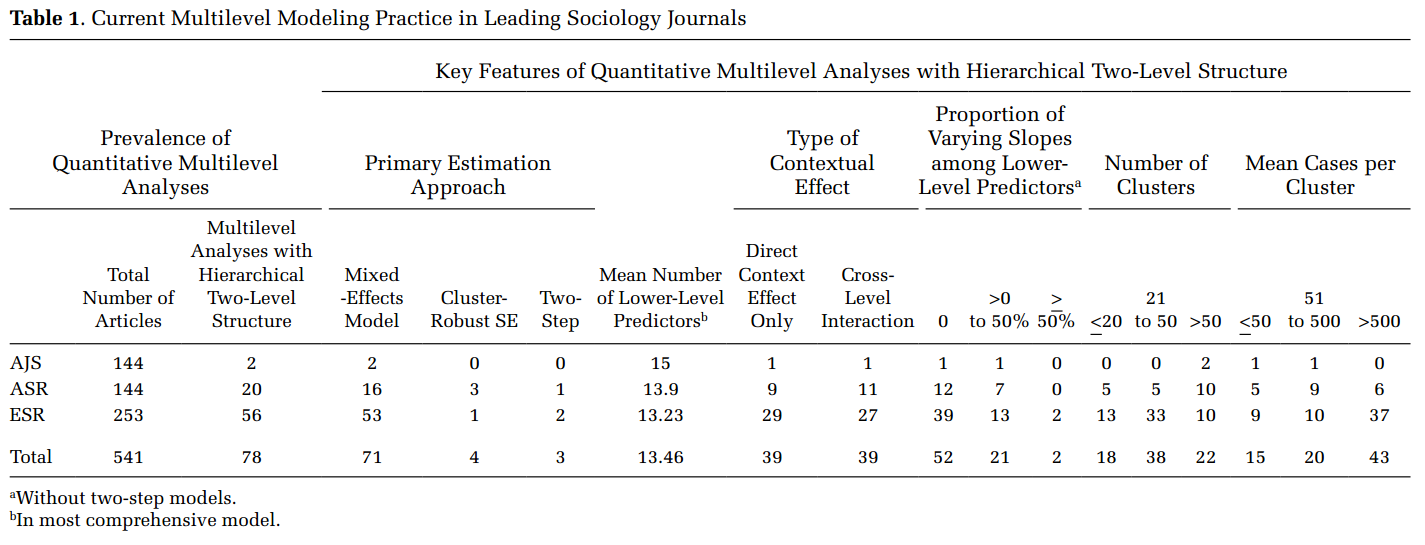
\includegraphics [scale=0.22]{mlm_research}
		  		\end{centering}
		  	\end{figure}

{\tiny 	(Heisig et al 2017)}

	\framebreak

	Multilevel models are used in sociology to specify the effect of social context
	on individual-level outcomes. The idea that individuals respond to their social
	context is a defining claim of the sociological discipline, which is found in
	Marx's work on political economy (1846), in Durkheim's studies of the impact
	of community on anomia and suicide (1897), in Weber's research on how
	religious communities shape economic behavior (1905), in Merton's work on
	communities, relative deprivation, and social comparison theory (1968), and
	in Berelson et aI's (1954) research into the effect of social context on voting.


	{\tiny 	(Diprete \& Forristal 1994)}

 \framebreak

		\begin{itemize}%[<+->] % este signo al lado del itemize es para las transiciones entre items
			\item Investigación sociológica y contexto
			\item Relaciones micro - macro: (una) posible operacionalización de relaciones entre contexto e individuo
		\end{itemize}
	\framebreak

	  	\begin{figure}[h]
	  		\begin{centering}
	  			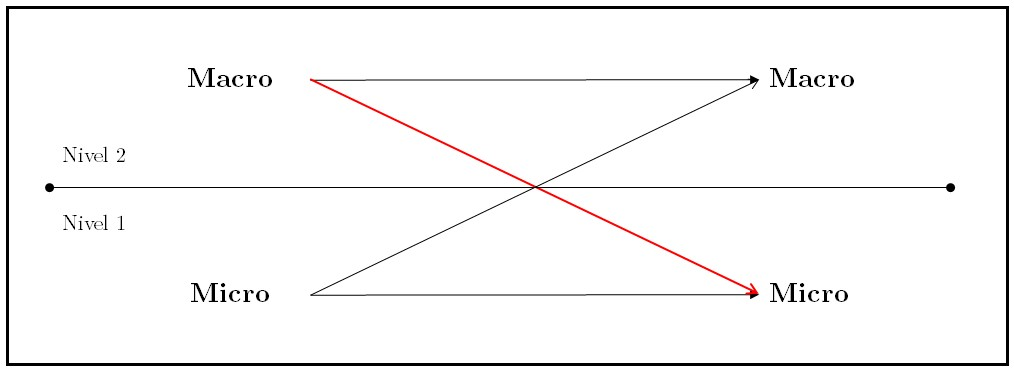
\includegraphics [scale=0.4]{macromicro}
	  		\end{centering}
	  	\end{figure}

	\framebreak

	  	\begin{figure}[h]
	  		\begin{centering}
	  			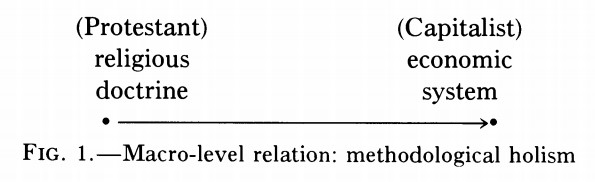
\includegraphics [scale=0.4]{coleman1macro}
	  		\end{centering}
	  \caption{\scriptsize Coleman, J. S. (1986). Social Theory, Social Research, and a Theory of Action. The American Journal of Sociology, 91(6), 1309–1335.}
	  	\end{figure}

	\framebreak

	\begin{figure}[h]
		\begin{centering}
			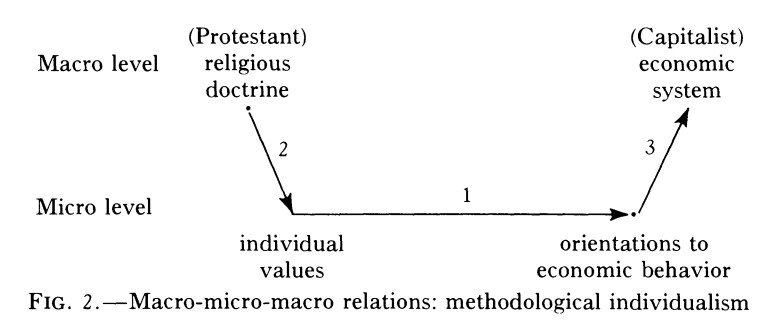
\includegraphics [scale=0.4]{coleman2macro}
		\end{centering}
	\caption{\scriptsize Coleman, J. S. (1986). Social Theory, Social Research, and a Theory of Action. The American Journal of Sociology, 91(6), 1309–1335.}
	\end{figure}


 \framebreak
	 Versiones del contexto
	 \begin{itemize}
		\item Variables macro - nivel 2 (Ejemplos: Países, comunas, escuelas, organizaciones)
		\item Tiempo
	\end{itemize}

	\end{frame}

\subsection{Falacia ecológica}
	\begin{frame}[allowframebreaks]{Outline}
		\frametitle{Falacia ecológica}
		Problemas asociados a la (des)consideración del contexto:
		\begin{itemize}%[<+->] % [<+->] para transiciones entre items
			\item Falacia ecológica: conclusiones erradas acerca de individuos basados en datos de contexto (macro)
			\item Ejemplo (ficticio): relación entre estatus socioeconómico e intención de voto
		\end{itemize}

	\framebreak

	  	\begin{figure}[h]
	  		\begin{centering}
	  			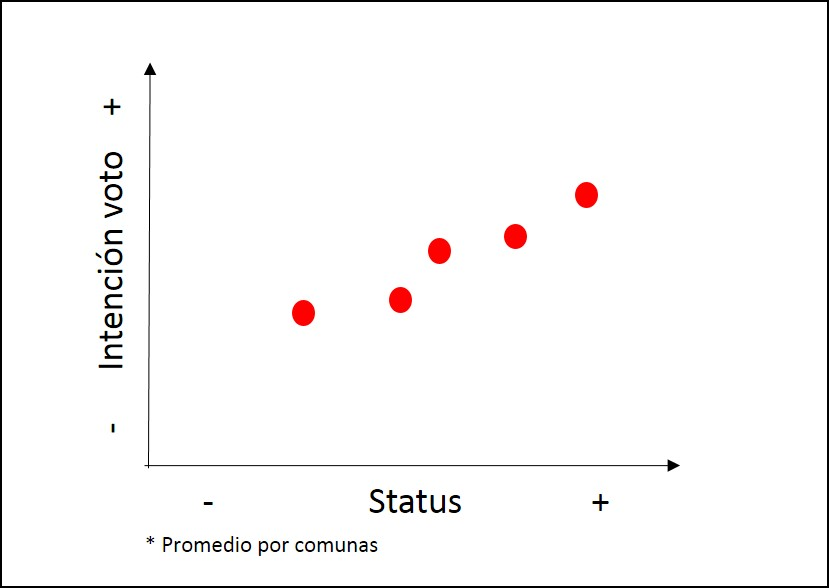
\includegraphics [scale=0.5]{fal1}
	  		\end{centering}
	  	\end{figure}

	  	\begin{figure}[h]
	  		\begin{centering}
	  			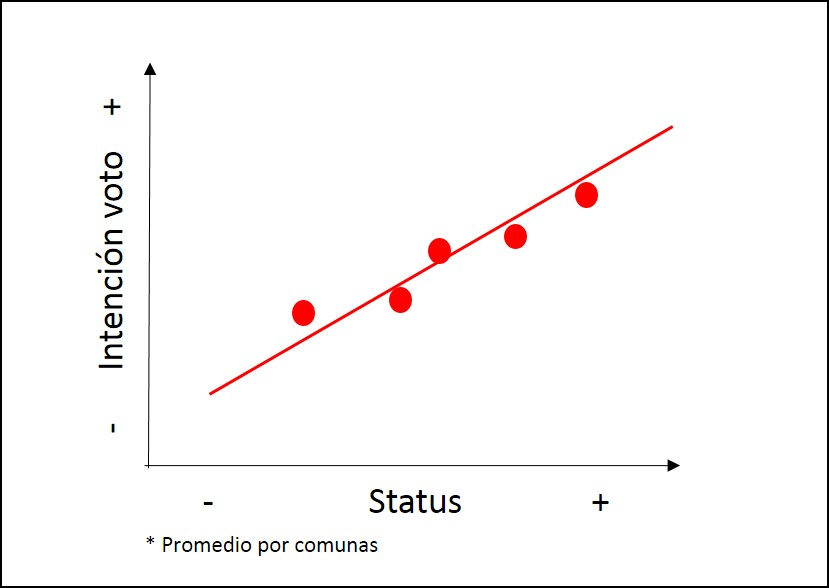
\includegraphics [scale=0.5]{fal2}
	  		\end{centering}
	  	\end{figure}

	  	\begin{figure}[h]
	  		\begin{centering}
	  			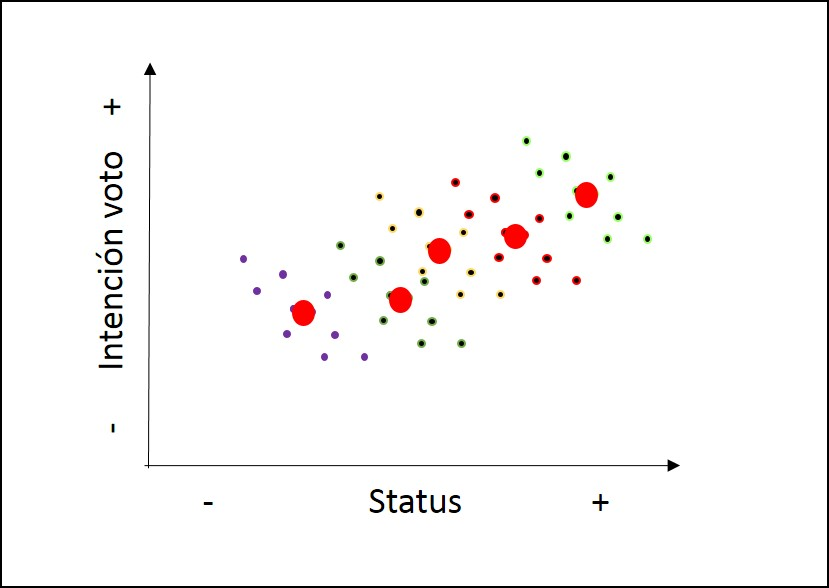
\includegraphics [scale=0.5]{fal3}
	  		\end{centering}
	  	\end{figure}

	  	\begin{figure}[h]
	  		\begin{centering}
	  			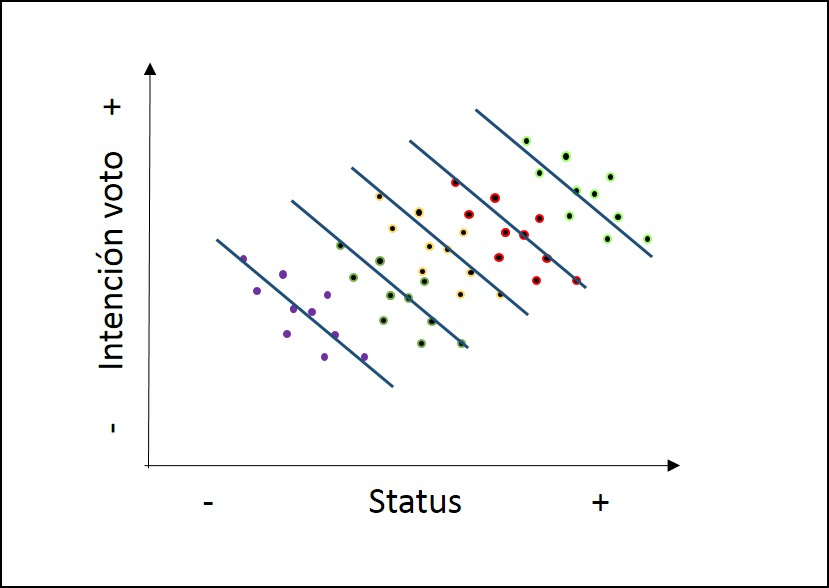
\includegraphics [scale=0.5]{fal4}
	  		\end{centering}
	  	\end{figure}

	  	\begin{figure}[h]
	  		\begin{centering}
	  			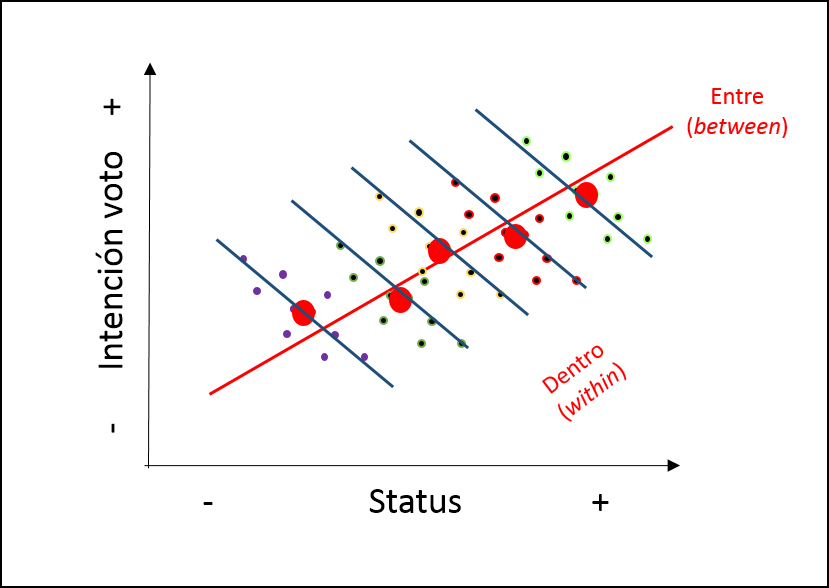
\includegraphics [scale=0.5]{fal5}
	  		\end{centering}
	  	\end{figure}

	\framebreak

	Implicancias
			\begin{itemize}%[<+->] % [<+->] para transiciones entre items
				\item Relaciones individuales y contextuales no necesariamente van en la misma dirección (lineal)
				\item Falacias también pueden ocurrir en la otra dirección (falacia individualista)
				\item  Por lo tanto la inferencia ecológica (contextual) no se corresponde necesariamente con la inferencia individual
				\item Falacia ecológica: caso extremo cuando ambas relaciones van en dirección contraria. No es lo usual, pero sirve como ilustración de diferencias within-between
				\item Distinguir ambos niveles es clave para estimación multinivel

			\framebreak

				\item Profundización falacia ecológica:
						\begin{itemize}%[<+->] % [<+->] para transiciones entre items
							\item Blakely, T. A., \& Woodward, A. J. (2000). Ecological effects in multi-level studies. Journal of Epidemiology and Community Health, 54(5), 367–374.

							\item Robinson W S 1950. Ecological correlations and the behavior of individuals. American Sociological
							Review 15: 351–57
						\end{itemize}
			\end{itemize}

	\end{frame}

\subsection{Contexto e implicancias}

	\begin{frame}%[allowframebreaks]{Outline}
		\frametitle{Contexto e implicancias teóricas}
		En el planteamiento de una investigación con hipótesis multinivel, es relevante definir:
		\begin{itemize}%[<+->] % este signo al lado del itemize es para las transiciones entre items
			\item Qué es el contexto
			\item Cuáles son los elementos principales del contexto a considerar en las hipótesis
			\item Cómo se relacionan variables del contexto con variables individuales (hipótesis)
		\end{itemize}
	\end{frame}

	\begin{frame}%[allowframebreaks]{Outline}
		\frametitle{Ejemplos}
		\begin{itemize}%[<+->] % este signo al lado del itemize es para las transiciones entre items
			\item Educación
			\item Opinión pública
			\item Participación política
		\end{itemize}
	\end{frame}

	\begin{frame}[allowframebreaks]{Outline}
		\frametitle{Contexto e implicancias estadísticas}
		\begin{itemize}%[<+->] % este signo al lado del itemize es para las transiciones entre items
			\item Estructuras de datos jerárquicos: variables nivel 1 (micro) y nivel 2 (macro)
			\item Implicancias estadísticas asociadas a incorporación de variables contextuales a modelos de regresión con datos individuales (dependencia contextual)
					\begin{enumerate}%[<+->] % [<+->] para transiciones entre items
						\item viola los supuestos de independencia de los residuos del modelo de regresión OLS (dependencia como "ruido")
						\item pero ... permite estudiar fenómenos que van más allá de hipótesis individuales (dependencia como fenómeno interesante)
					\end{enumerate}

		\framebreak

			\item Por lo tanto, los modelos multinivel tienen dos sentidos principales a nivel estadístico:
					\begin{itemize}%[<+->] % [<+->] para transiciones entre items
						\item Corregir estimaciones con variables individuales cuando existe dependencia contextual (disminuye el error)
						\item Hace posible contrastar hipótesis que abarcan relaciones entre niveles
					\end{itemize}


		\end{itemize}
	\end{frame}

\section{Modelos multinivel}

	\begin{frame}%[allowframebreaks]{Outline}
		\begin{minipage}{\textwidth} % con esta instruccion para ajustar espacio entre líneas
			\tableofcontents  [currentsection,currentsubsection]
		\end{minipage}
	\end{frame}


	\begin{frame}%[allowframebreaks]{Outline}
	\frametitle{Modelos multinivel}

			\begin{itemize}%[<+->] % [<+->] para transiciones entre items
				\item Definición minimalista: modelos de regresión que incluyen variables individuales y contextuales, reconociendo la estructura jerárquica/anidada en la estimación y permitiendo contrastar hipótesis que relacionan variables individuales y contextuales
				\item Otras versiones: modelos jerárquicos, modelos mixtos, modelos contextuales, modelos con efectos aleatorios
			\end{itemize}
	\end{frame}

	\begin{frame}[allowframebreaks]{Outline}
	\frametitle{Tipos generales de problemas multinivel}

	Tres tipos de preguntas básicas, ejemplo educación:
	\begin{enumerate}%[<+->] % signo [<+->] para las transiciones entre items
		\item ¿Existen diferencias de rendimiento académico de los alumnos entre escuelas?
		\item ¿Tienen estas diferencias relación con variables de la escuela?
		\item Las características de los estudiantes, ¿poseen un efecto distinto en rendimiento de acuerdo a características de las escuelas?
	\end{enumerate}

\end{frame}

	\begin{frame}[allowframebreaks]{Outline}
		\frametitle{Tipos generales de estimaciones multinivel}

	Base: modelo de regresión simple (no multinivel)
	  	\begin{figure}[h]
	  		\begin{centering}
	  			
\includegraphics [scale=0.8]{mod1}
	  		\end{centering}
	  	\end{figure}

	\framebreak

	Modelo multinivel con predictores individuales
	\begin{figure}[h]
		\begin{centering}
			
\includegraphics [scale=0.8]{mod2}
		\end{centering}
	\end{figure}

	\framebreak

	Modelo multinivel con predictores contextuales
	\begin{figure}[h]
		\begin{centering}
			
\includegraphics [scale=0.8]{mod3}
		\end{centering}
	\end{figure}

	\framebreak

	MModelo multinivel con predictores individuales y contextuales
	\begin{figure}[h]
		\begin{centering}
			
\includegraphics [scale=0.8]{mod4}
		\end{centering}
	\end{figure}

	\framebreak

	Modelo multinivel con interacción entre niveles
	\begin{figure}[h]
		\begin{centering}
			
\includegraphics [scale=0.8]{mod5}
		\end{centering}
	\end{figure}

	\framebreak


	(A detallar próxima clase - abriendo esquemas)

	\begin{enumerate}%[<+->] % este signo al lado del itemize es para las transiciones entre items

		\item Correlación intra clase
		\item Estimación con predictores nivel 1 (ajustando por anidación)
		\item (multiples) predictores nivel 2
		\item Variabilidad de parámetros de estimación nivel 1 (pendientes)
		\item Interacción entre niveles
	\end{enumerate}
   \end{frame}

	\begin{frame}%[allowframebreaks]{Outline}
		\frametitle{Resumen}
		\begin{itemize}%[<+->] % [<+->] para transiciones entre items
			\item Contexto en sociología
			\item Extensión del modelo de regresión simple
			\item Distintos problemas de investigación multinivel
			\item Aplicaciones en distintos ámbitos y disciplinas
			\item Diferencia entre nivel individual y contextual (witihin/between)
			\item Extiende posibilidades de estimación, permitiendo contrastar hipótesis más complejas de relaciones micro/macro
		\end{itemize}
	\end{frame}


%========================================================
\againframe[plain]{firstframe} % repite slide inicial

\end{document}

 % Basic frame

	\begin{frame}%[allowframebreaks]{Outline}
	\frametitle{XX}
  	\begin{itemize}%[<+->] % este signo al lado del itemize es para las transiciones entre items
  	\item
  	\item
    \end{itemize}
	\end{frame}

	\note [itemize]{
	\item I
	}

<1-> : después de \item permite ordenar el orden de aparición según el número

% Insertar figuras
  	\begin{figure}[h]
	\begin{centering}
	\includegraphics [scale=0.1]{simon}
	\end{centering}
	\end{figure}


% Figuras a la derecha del texto

    \begin{columns}
    	\column{0.30\linewidth}
        \centering
        \includegraphics[scale=0.35]{aqui imagen}
        \column{0.70 \linewidth}
		\textbf{titulo del texto a la derecha}
		\begin{itemize}
			\item XX
	\end{itemize}
    \end{columns}

% weblinks
\href{https://www.statmodel.com}{\beamergotobutton{www}}
